% \documentclass[../../main.tex]{subfiles}

\begin{document}
\pagebreak
 \subsubsection{Heltec Lora32}

\begin{wrapfigure}[8]{l}[-8mm]{0.28\textwidth}
    \centering
    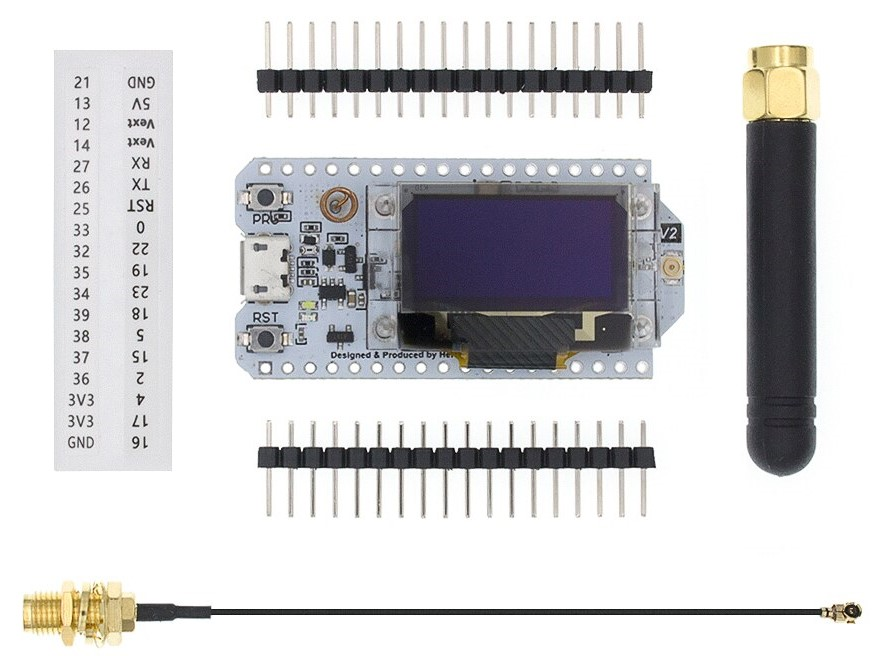
\includegraphics[width=0.27\textwidth]{images/heltec_lora32.jpg}
    \caption{ vývojová doska Wifi LoRa32  }
\end{wrapfigure}
Wifi LoRa 32 je IoT vývojová doska integrovaná s ESP32 + SX127x. Má Wi-Fi, BLE, LoRa funkcie, Li-Po systém manažmentu batérie, 0.96 palca OLED, Micro USB rozhranie s regulátorom napätia, ochranu proti elektrostatickému výboju a ďalšie ochrany, platný certifikát CE Certificate\cite{heltec_lora32}.
\paragraph{MicroPython}
Je to impelementácia programovacieho jazyka Python 3 optimalizovaná na beh v mikrokontroléroch.\cite{micropython_pcrevue}. Je to Interpretovaný jazyk. Má zabudovaný prompt REPL pre okamžité vykonávanie príkazov. Podporuje veľa architektúr (x86, x86-64, ARM, ARM Thumb, Xtensa)\cite{micropython}

% \bigskip
% \bigskip

% SX1276-SX1278-ESP32-LoRa-868MHz-915MHz-433MHz-0-96-Inch-Blue-OLED-Display-Bluetooth-WIFI-



% \vfill

\end{document}